\documentclass[12pt]{article}
\usepackage{fancyhdr}
\usepackage{amsmath,amsfonts,enumerate}
\usepackage{color,graphicx}
\usepackage{tikz}
\usepackage{pgfplots}
\usepackage{listings}
\usepackage{algorithm}
\usepackage{algorithmic}
\usetikzlibrary{arrows,positioning,shapes,calc,matrix}
\pagestyle{fancy}

% Define colors for answers
\definecolor{answercolor}{RGB}{0,100,0}
\definecolor{explanationcolor}{RGB}{0,0,139}

% Custom commands for answers
\newcommand{\answer}[1]{{\color{answercolor}\textbf{Answer:} #1}}
\newcommand{\explanation}[1]{{\color{explanationcolor}#1}}

%%%%%%%%%%%%%%%%%%%%%%%%%%%%%%%%%%%%%%%%%%%%%%%%%
% Course customization based on Professor's teaching
%%%%%%%%%%%%%%%%%%%%%%%%%%%%%%%%%%%%%%%%%%%%%%%%%
\newcommand{\masunitnumber}{CENG 403}
\newcommand{\examdate}{January 2025}
\newcommand{\academicyear}{2024-2025}
\newcommand{\semester}{I}
\newcommand{\coursename}{Deep Learning - CNN Architectures \& RNN Introduction - ANSWERED}
\newcommand{\numberofhours}{3}
%%%%%%%%%%%%%%%%%%%%%%%%%%%%%%%%%%%%%%%%%%%%%%%%%
% CUSTOM SPACING COMMANDS FOR ANSWER SPACES
%%%%%%%%%%%%%%%%%%%%%%%%%%%%%%%%%%%%%%%%%%%%%%%%%
\newcommand{\answerspace}[1]{\vspace{#1}}
\newcommand{\questionspace}{\vspace{3cm}}        
\newcommand{\subquestionspace}{\vspace{2.5cm}}   
\newcommand{\shortanswer}{\vspace{2cm}}          
\newcommand{\mediumanswer}{\vspace{3cm}}         
\newcommand{\longanswer}{\vspace{4cm}}           
\newcommand{\journalspace}{\vspace{4.5cm}}       
\newcommand{\codespace}{\vspace{5cm}}            
%%%%%%%%%%%%%%%%%%%%%%%%%%%%%%%%%%%%%%%%%%%%%%%%%
% Header setup
%%%%%%%%%%%%%%%%%%%%%%%%%%%%%%%%%%%%%%%%%%%%%%%%%
\lhead{}
\rhead{}
\chead{{\bf MIDDLE EAST TECHNICAL UNIVERSITY}}
\lfoot{}
\rfoot{}
\cfoot{}
\begin{document}
\setlength{\headsep}{5truemm}
\setlength{\headheight}{14.5truemm}
\setlength{\voffset}{-0.45truein}
\renewcommand{\headrulewidth}{0.0pt}
\begin{center}
SEMESTER \semester\ EXAMINATION \academicyear
\end{center}
\begin{center}
{\bf \masunitnumber\ -- \coursename}
\end{center}
\vspace{20truemm}
\noindent \examdate\hspace{45truemm} TIME ALLOWED: \numberofhours\ HOURS
\vspace{19truemm}
\hrule
\vspace{19truemm}
\noindent\underline{INSTRUCTIONS TO CANDIDATES}
\vspace{8truemm}
%%%%%%%%%%%%%%%%%%%%%%%%%%%%%%%%%%%%%%%%%%%%%%%%%%%%%%
% Instructions based on professor's emphasis
%%%%%%%%%%%%%%%%%%%%%%%%%%%%%%%%%%%%%%%%%%%%%%%%%%%%%%
\begin{enumerate}
\item This examination paper contains {\bf SIX (6)} questions and comprises 
{\bf EIGHT (8)} printed pages.
\item Answer all questions. 
The marks for each question are indicated at the beginning of each question.
\item Answer each question beginning on a {\bf FRESH} page of the answer book.
\item This {\bf IS NOT an OPEN BOOK} exam.
\item Show clear reasoning for your answers, especially intuitive explanations.
\item For architectural diagrams, draw clear components and explain design choices.
\item Connect concepts to examples discussed in lectures where relevant.
\item Explain the practical implications of design decisions.
\end{enumerate}
%%%%%%%%%%%%%%%%%%%%%%%%%%%%%%%%%%%%%%%%%%%%%%%%%
% New page for questions
%%%%%%%%%%%%%%%%%%%%%%%%%%%%%%%%%%%%%%%%%%%%%%%%%
\newpage
\lhead{}
\rhead{\masunitnumber}
\chead{}
\lfoot{}
\cfoot{\thepage}
\rfoot{}
\setlength{\footskip}{45pt}
%%%%%%%%%%%%%%%%%%%%%%%%%%%%%%%%%%%%%%%%%%%%%%%%%%
% EXAM QUESTIONS BASED ON PROFESSOR'S TEACHING
%%%%%%%%%%%%%%%%%%%%%%%%%%%%%%%%%%%%%%%%%%%%%%%%%%

\paragraph{Question 1. ResNet and Skip Connections}{\hfill (25 marks)}\\
Based on the professor's explanation: "The identity function doesn't have to be learned as part of the solution, we are giving identity as part of the solution."

\begin{enumerate}[(a)]
    \item The professor mentioned that ResNet researchers "noticed that up to a certain number of layers actually performance degrades." Explain why this was counterintuitive and how skip connections solve this problem. Include the professor's explanation of why networks have difficulty learning the identity function. \hfill (8 marks)
    
    \answer{The degradation problem was counterintuitive because adding more layers should theoretically allow networks to learn at least as good a representation as the shallower network by learning identity mappings in the additional layers.}
    
    \explanation{
    The professor explained this counterintuitive finding in detail:
    
    \textbf{Why degradation was unexpected:}
    \begin{itemize}
        \item Deeper networks should have at least the same representational capacity as shallower ones
        \item If additional layers learn identity functions, performance should not degrade
        \item The issue wasn't overfitting (since both training and test error increased)
    \end{itemize}
    
    \textbf{The core problem:} Networks have difficulty learning the identity function because:
    \begin{itemize}
        \item Identity mapping $H(x) = x$ seems simple but is actually hard to learn through composition of ReLU and linear layers
        \item Multiple non-linear layers struggle to approximate the identity transformation
        \item Gradient vanishing makes it difficult for deep layers to receive useful learning signals
    \end{itemize}
    
    \textbf{How skip connections solve this:}
    \begin{itemize}
        \item Instead of learning $H(x)$, the network learns residual $F(x) = H(x) - x$
        \item Then $H(x) = F(x) + x$, where identity is built into the architecture
        \item If the optimal function is close to identity, $F(x)$ approaches zero, which is easier to learn
        \item The identity path is always preserved, providing a baseline performance guarantee
    \end{itemize}
    }
    
    \item Draw a ResNet block as described by the professor, showing how "in forward pass the identity can be implemented as part of the solution" and "in backward pass through these residual connections gradient can flow without any vanishing issues." \hfill (10 marks)
    
    \begin{center}
    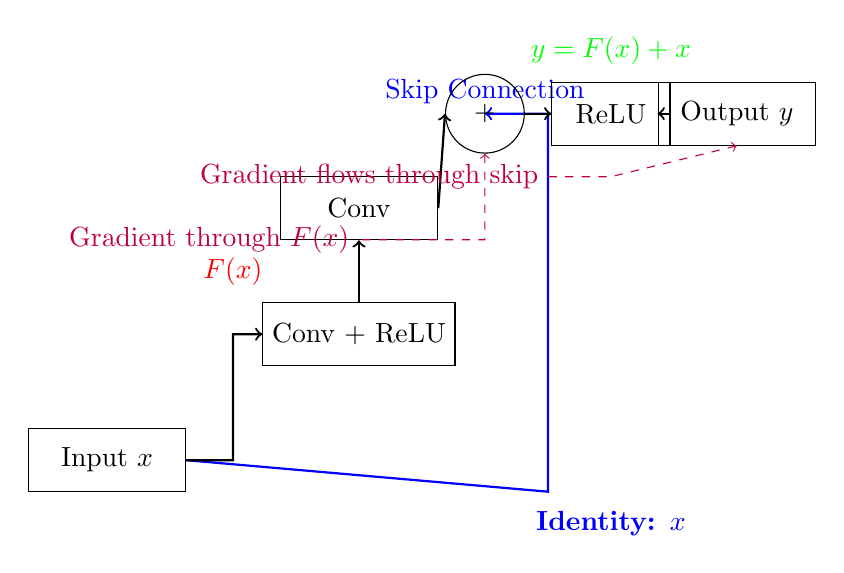
\begin{tikzpicture}[scale=0.8]
        % Input
        \node[draw, rectangle, minimum width=2cm, minimum height=0.8cm] (input) at (0,0) {Input $x$};
        
        % Main path - weight layers
        \node[draw, rectangle, minimum width=2cm, minimum height=0.8cm] (conv1) at (4,2) {Conv + ReLU};
        \node[draw, rectangle, minimum width=2cm, minimum height=0.8cm] (conv2) at (4,4) {Conv};
        
        % Skip connection
        \draw[thick, blue, ->] (input.east) -- (7,-0.5) -- (7,5.5) -- (6,5.5) node[above, blue] {Skip Connection};
        
        % Main path connections
        \draw[thick, ->] (input.east) -- (2,0) -- (2,2) -- (conv1.west);
        \draw[thick, ->] (conv1.north) -- (conv2.south);
        
        % Addition
        \node[draw, circle, minimum size=1cm] (add) at (6,5.5) {$+$};
        \draw[thick, ->] (conv2.east) -- (add.west);
        
        % ReLU after addition
        \node[draw, rectangle, minimum width=1.5cm, minimum height=0.8cm] (relu) at (8,5.5) {ReLU};
        \draw[thick, ->] (add.east) -- (relu.west);
        
        % Output
        \node[draw, rectangle, minimum width=2cm, minimum height=0.8cm] (output) at (10,5.5) {Output $y$};
        \draw[thick, ->] (relu.east) -- (output.west);
        
        % Labels
        \node[red] at (2,3) {\textbf{$F(x)$}};
        \node[blue] at (8,-1) {\textbf{Identity: $x$}};
        \node[green] at (8,6.5) {\textbf{$y = F(x) + x$}};
        
        % Gradient flow illustration
        \draw[dashed, purple, <-] (output.south) -- (8,4.5) -- (7,4.5) node[left, purple] {Gradient flows through skip};
        \draw[dashed, purple, <-] (add.south) -- (6,3.5) -- (4,3.5) node[left, purple] {Gradient through $F(x)$};
    \end{tikzpicture}
    \end{center}
    
    \explanation{
    \textbf{Forward Pass (Identity Implementation):}
    \begin{itemize}
        \item Input $x$ splits into two paths: identity path and weight layers path
        \item Weight layers compute $F(x)$ (the residual function)
        \item Identity path preserves original input $x$ unchanged
        \item Output: $y = F(x) + x$ combines both paths
    \end{itemize}
    
    \textbf{Backward Pass (Gradient Flow):}
    \begin{itemize}
        \item Gradient $\frac{\partial L}{\partial y}$ reaches the addition node
        \item Splits into two paths: $\frac{\partial L}{\partial F(x)}$ and $\frac{\partial L}{\partial x}$
        \item Identity path: $\frac{\partial L}{\partial x} = \frac{\partial L}{\partial y} \cdot 1 = \frac{\partial L}{\partial y}$
        \item This ensures at least one gradient path is never vanishing (always has magnitude 1)
        \item Even if $F(x)$ gradients vanish, identity gradients flow unimpeded
    \end{itemize}
    }
    
    \item The professor explained that ResNet "smooths the loss surface" and provides "robustness to slight changes in the weights." Explain this concept using the professor's reasoning about how identity transform provides robustness when weights change slightly. \hfill (7 marks)
    
    \answer{The identity transform in ResNet provides inherent robustness because even if the learned weights $F(x)$ become suboptimal due to slight changes, the identity path $x$ always preserves the original input, creating a safety net that smooths the loss landscape.}
    
    \explanation{
    \textbf{Loss Surface Smoothing:}
    \begin{itemize}
        \item Traditional deep networks have sharp, non-convex loss surfaces
        \item Small weight changes can lead to large performance drops
        \item ResNet's identity connections create "highways" in the loss landscape
        \item These highways provide consistent paths even when weights change
    \end{itemize}
    
    \textbf{Robustness Mechanism:}
    \begin{itemize}
        \item If weights in $F(x)$ become slightly perturbed: $F'(x) = F(x) + \delta F(x)$
        \item Output becomes: $y' = F'(x) + x = F(x) + \delta F(x) + x$
        \item The identity term $x$ remains unchanged, providing stability
        \item Even if $\delta F(x)$ is large, the identity ensures reasonable output
    \end{itemize}
    
    \textbf{Mathematical Insight:}
    \begin{itemize}
        \item The Jacobian $\frac{\partial y}{\partial x} = \frac{\partial F(x)}{\partial x} + I$ always has identity component
        \item This prevents the Jacobian from becoming arbitrarily small or large
        \item Results in more stable training dynamics and better generalization
        \item Creates multiple viable paths through the network, increasing robustness
    \end{itemize}
    }
\end{enumerate}

\newpage
\paragraph{Question 2. ResNeXt and Multiple Pathways}{\hfill (20 marks)}\\
The professor described ResNeXt as extending ResNet "by utilizing multiple paths acting on the same input layer."

\begin{enumerate}[(a)]
    \item Compare ResNeXt with the inception module from GoogleNet as the professor discussed. Explain the key difference: "in inception module the filter sizes are different in different paths, whereas here in ResNeXt the sizes are the same." \hfill (8 marks)
    
    \answer{ResNeXt and Inception modules both use multiple parallel paths, but ResNeXt uses identical transformations across all paths while Inception uses different filter sizes to capture multi-scale information.}
    
    \explanation{
    \textbf{Inception Module Approach:}
    \begin{itemize}
        \item Multiple paths with different receptive field sizes: 1×1, 3×3, 5×5 convolutions
        \item Each path captures information at different scales
        \item Designed to handle the "what size should my filter be?" problem
        \item Concatenates outputs from different-sized filters
    \end{itemize}
    
    \textbf{ResNeXt Approach:}
    \begin{itemize}
        \item Multiple paths with identical transformations: same filter sizes across all paths
        \item Each path learns different feature representations using same architecture
        \item Focuses on "how many transformations should I apply?" rather than "what size?"
        \item Aggregates outputs from same-sized but differently-trained filters
    \end{itemize}
    
    \textbf{Key Philosophical Difference:}
    \begin{itemize}
        \item Inception: \textit{Diversity through different scales}
        \item ResNeXt: \textit{Diversity through multiple identical transformations}
        \item Inception targets multi-scale feature extraction
        \item ResNeXt targets ensemble-like behavior within a single block
    \end{itemize}
    }
    
    \item The professor noted that ResNeXt "can provide better performance than ResNet however because of the multiple paths it is slower." Explain this trade-off and when you would choose ResNeXt over ResNet according to the professor's guidance. \hfill (7 marks)
    
    \answer{ResNeXt provides better accuracy through ensemble-like multiple pathways but requires more computation. Choose ResNeXt when accuracy is critical and computational resources are available; choose ResNet when speed and efficiency are priorities.}
    
    \explanation{
    \textbf{Performance Advantage:}
    \begin{itemize}
        \item Multiple paths create ensemble-like behavior within single blocks
        \item Each path can specialize in different aspects of feature learning
        \item Aggregation of multiple transformations reduces variance
        \item Better generalization through implicit regularization
    \end{itemize}
    
    \textbf{Computational Cost:}
    \begin{itemize}
        \item ResNeXt requires computing multiple parallel transformations
        \item Memory usage increases proportional to cardinality (number of paths)
        \item Cannot fully utilize parallel computing due to aggregation step
        \item Approximately C times slower than ResNet (where C = cardinality)
    \end{itemize}
    
    \textbf{When to Choose Each:}
    \begin{itemize}
        \item \textbf{Choose ResNeXt:} High-accuracy applications (medical imaging, autonomous vehicles), sufficient computational budget, offline processing
        \item \textbf{Choose ResNet:} Real-time applications, mobile/edge devices, limited computational resources, online inference
    \end{itemize}
    }
    
    \item Draw a ResNeXt block showing multiple functions $f_1(x), f_2(x), \ldots, f_{32}(x)$ acting on the same input as the professor illustrated, resulting in $x + f_1(x) + f_2(x) + \ldots + f_{32}(x)$. \hfill (5 marks)
    
    \begin{center}
    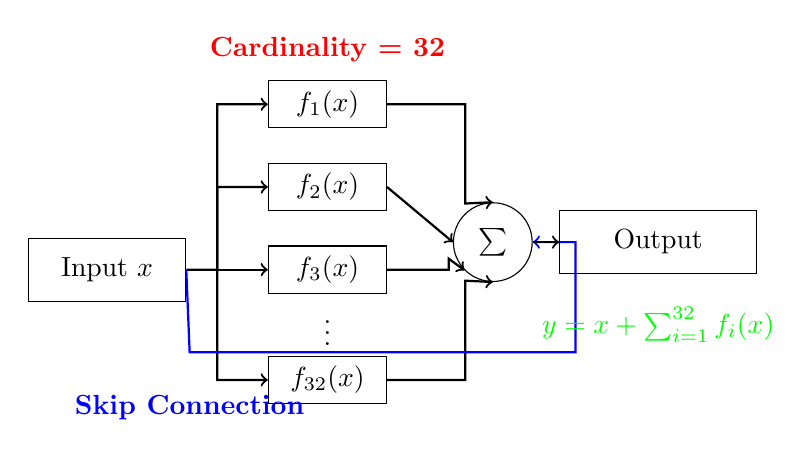
\begin{tikzpicture}[scale=0.7]
        % Input
        \node[draw, rectangle, minimum width=2cm, minimum height=0.8cm] (input) at (0,0) {Input $x$};
        
        % Multiple paths
        \node[draw, rectangle, minimum width=1.5cm, minimum height=0.6cm] (f1) at (4,3) {$f_1(x)$};
        \node[draw, rectangle, minimum width=1.5cm, minimum height=0.6cm] (f2) at (4,1.5) {$f_2(x)$};
        \node[draw, rectangle, minimum width=1.5cm, minimum height=0.6cm] (f3) at (4,0) {$f_3(x)$};
        \node at (4,-1) {\vdots};
        \node[draw, rectangle, minimum width=1.5cm, minimum height=0.6cm] (f32) at (4,-2) {$f_{32}(x)$};
        
        % Connections from input to all paths
        \draw[thick, ->] (input.east) -- (2,0) -- (2,3) -- (f1.west);
        \draw[thick, ->] (2,0) -- (2,1.5) -- (f2.west);
        \draw[thick, ->] (2,0) -- (f3.west);
        \draw[thick, ->] (2,0) -- (2,-2) -- (f32.west);
        
        % Aggregation
        \node[draw, circle, minimum size=1cm] (sum) at (7,0.5) {$\sum$};
        \draw[thick, ->] (f1.east) -- (6.5,3) -- (6.5,1.2) -- (sum.north);
        \draw[thick, ->] (f2.east) -- (sum.west);
        \draw[thick, ->] (f3.east) -- (6.2,0) -- (6.2,0.2) -- (sum.south west);
        \draw[thick, ->] (f32.east) -- (6.5,-2) -- (6.5,-0.2) -- (sum.south);
        
        % Skip connection
        \draw[thick, blue, ->] (input.east) -- (1.5,-1.5) -- (8.5,-1.5) -- (8.5,0.5) -- (sum.east);
        
        % Output
        \node[draw, rectangle, minimum width=2.5cm, minimum height=0.8cm] (output) at (10,0.5) {Output};
        \draw[thick, ->] (sum.east) -- (output.west);
        
        % Labels
        \node[red] at (4,4) {\textbf{Cardinality = 32}};
        \node[blue] at (1.5,-2.5) {\textbf{Skip Connection}};
        \node[green] at (10,-1) {\textbf{$y = x + \sum_{i=1}^{32} f_i(x)$}};
    \end{tikzpicture}
    \end{center}
    
    \explanation{
    \textbf{ResNeXt Block Structure:}
    \begin{itemize}
        \item Input $x$ is fed to 32 identical transformation functions
        \item Each $f_i(x)$ has same architecture but different learned parameters
        \item All transformations are computed in parallel
        \item Outputs are aggregated through element-wise addition
        \item Skip connection adds original input to aggregated result
        \item Final output: $y = x + \sum_{i=1}^{32} f_i(x)$
    \end{itemize}
    }
\end{enumerate}

\newpage
\paragraph{Question 3. DenseNet Architecture}{\hfill (22 marks)}\\
Based on the professor's explanation: "We have residual connections not only skipping the next block but skipping to and making connections to all following blocks."

\begin{enumerate}[(a)]
    \item Explain DenseNet's approach to skip connections as described by the professor. Why does having "skip connections for all following layers" make it "a very dense network" and potentially "more difficult to implement"? \hfill (8 marks)
    
    \answer{DenseNet creates skip connections from each layer to ALL subsequent layers, creating a dense connectivity pattern where layer $\ell$ receives feature maps from all preceding layers $0, 1, 2, \ldots, \ell-1$, making implementation complex due to the quadratic growth in connections.}
    
    \explanation{
    \textbf{DenseNet Connectivity Pattern:}
    \begin{itemize}
        \item Layer $\ell$ receives inputs from layers $0, 1, 2, \ldots, \ell-1$
        \item Each layer's input: $x_\ell = H_\ell([x_0, x_1, \ldots, x_{l-1}])$
        \item $[x_0, x_1, \ldots, x_{l-1}]$ represents concatenation of all previous feature maps
        \item Creates $\frac{L(L+1)}{2}$ connections for $L$ layers (quadratic growth)
    \end{itemize}
    
    \textbf{Why it's "Very Dense":}
    \begin{itemize}
        \item Every layer connects to every other layer in a feed-forward fashion
        \item Information flows directly from any layer to all subsequent layers
        \item Creates maximum information flow density possible
        \item Results in rich feature reuse and gradient flow
    \end{itemize}
    
    \textbf{Implementation Difficulties:}
    \begin{itemize}
        \item Memory complexity: Each layer must store and access all previous feature maps
        \item Concatenation operations become increasingly expensive
        \item GPU memory management becomes challenging
        \item Requires careful memory optimization to avoid out-of-memory errors
        \item Debugging and visualization become complex due to dense connections
    \end{itemize}
    }
    
    \item The professor mentioned that DenseNet "can provide better performance compared to ResNet" but wasn't sure "why it didn't become as popular as ResNet." Analyze the potential reasons for this based on implementation complexity and computational requirements. \hfill (8 marks)
    
    \answer{Despite better performance, DenseNet's popularity was limited by implementation complexity, memory requirements, computational overhead of concatenation operations, and the practical simplicity advantage of ResNet's architecture.}
    
    \explanation{
    \textbf{Performance Advantages of DenseNet:}
    \begin{itemize}
        \item Better parameter efficiency (fewer parameters for same performance)
        \item Stronger gradient flow due to direct connections
        \item Implicit regularization through feature reuse
        \item Better feature propagation and reuse
    \end{itemize}
    
    \textbf{Reasons for Limited Adoption:}
    
    \textbf{1. Memory Constraints:}
    \begin{itemize}
        \item Memory usage grows quadratically with depth
        \item GPU memory limitations restrict practical network sizes
        \item Batch size limitations reduce training efficiency
    \end{itemize}
    
    \textbf{2. Implementation Complexity:}
    \begin{itemize}
        \item Requires sophisticated memory management
        \item Concatenation operations are computationally expensive
        \item More complex to implement efficiently in frameworks
        \item Harder to optimize for different hardware
    \end{itemize}
    
    \textbf{3. Practical Considerations:}
    \begin{itemize}
        \item ResNet's simplicity makes it easier to modify and extend
        \item ResNet has cleaner mathematical formulation
        \item Industry adoption favored simpler, more reliable architectures
        \item Transfer learning and fine-tuning are simpler with ResNet
    \end{itemize}
    }
    
    \item Draw a DenseNet block showing how "from this layer we have skip connections to all following layers" as the professor described. Show at least 4 layers with their dense connections. \hfill (6 marks)
    
    \begin{center}
    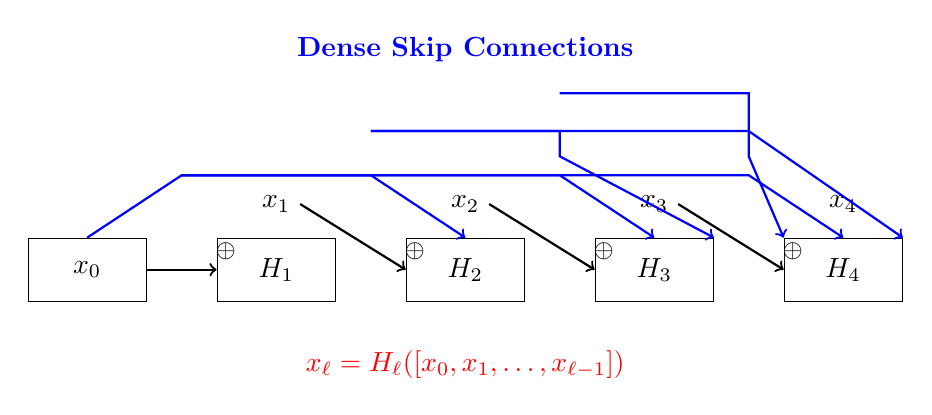
\begin{tikzpicture}[scale=0.8]
        % Input
        \node[draw, rectangle, minimum width=1.5cm, minimum height=0.8cm] (x0) at (0,0) {$x_0$};
        
        % Layers
        \node[draw, rectangle, minimum width=1.5cm, minimum height=0.8cm] (h1) at (3,0) {$H_1$};
        \node[draw, rectangle, minimum width=1.5cm, minimum height=0.8cm] (h2) at (6,0) {$H_2$};
        \node[draw, rectangle, minimum width=1.5cm, minimum height=0.8cm] (h3) at (9,0) {$H_3$};
        \node[draw, rectangle, minimum width=1.5cm, minimum height=0.8cm] (h4) at (12,0) {$H_4$};
        
        % Feature maps
        \node[above=0.2cm of h1] (x1) {$x_1$};
        \node[above=0.2cm of h2] (x2) {$x_2$};
        \node[above=0.2cm of h3] (x3) {$x_3$};
        \node[above=0.2cm of h4] (x4) {$x_4$};
        
        % Dense connections
        % To H1
        \draw[thick, ->] (x0.east) -- (h1.west);
        
        % To H2
        \draw[thick, blue, ->] (x0.north) -- (1.5,1.5) -- (4.5,1.5) -- (h2.north);
        \draw[thick, ->] (x1.east) -- (h2.west);
        
        % To H3
        \draw[thick, blue, ->] (1.5,1.5) -- (7.5,1.5) -- (h3.north);
        \draw[thick, blue, ->] (4.5,2.2) -- (7.5,2.2) -- (7.5,1.8) -- (h3.north east);
        \draw[thick, ->] (x2.east) -- (h3.west);
        
        % To H4
        \draw[thick, blue, ->] (1.5,1.5) -- (10.5,1.5) -- (h4.north);
        \draw[thick, blue, ->] (4.5,2.2) -- (10.5,2.2) -- (10.5,1.8) -- (h4.north west);
        \draw[thick, blue, ->] (7.5,2.8) -- (10.5,2.8) -- (10.5,2.2) -- (h4.north east);
        \draw[thick, ->] (x3.east) -- (h4.west);
        
        % Labels
        \node[blue] at (6,3.5) {\textbf{Dense Skip Connections}};
        \node[red] at (6,-1.5) {\textbf{$x_\ell = H_\ell([x_0, x_1, \ldots, x_{\ell-1}])$}};
        
        % Concatenation symbols
        \node at (2.2,0.3) {\small $\oplus$};
        \node at (5.2,0.3) {\small $\oplus$};
        \node at (8.2,0.3) {\small $\oplus$};
        \node at (11.2,0.3) {\small $\oplus$};
    \end{tikzpicture}
    \end{center}
    
    \explanation{
    \textbf{Dense Connection Pattern:}
    \begin{itemize}
        \item $x_1 = H_1(x_0)$ - Layer 1 receives only $x_0$
        \item $x_2 = H_2([x_0, x_1])$ - Layer 2 receives concatenation of $x_0$ and $x_1$
        \item $x_3 = H_3([x_0, x_1, x_2])$ - Layer 3 receives all previous feature maps
        \item $x_4 = H_4([x_0, x_1, x_2, x_3])$ - Layer 4 receives all previous feature maps
    \end{itemize}
    
    \textbf{Key Features:}
    \begin{itemize}
        \item Blue arrows show skip connections bypassing multiple layers
        \item $\oplus$ symbols represent concatenation operations
        \item Each layer's input grows with network depth
        \item Maximum information reuse and gradient flow
    \end{itemize}
    }
\end{enumerate}

\newpage
\paragraph{Question 4. Highway Networks and Gating}{\hfill (23 marks)}\\
The professor explained highway networks as providing "more flexibility to the network where we can modulate the skip connection."

\begin{enumerate}[(a)]
    \item Explain the highway network concept as described by the professor: "multiply the skip connection by a learnable function" and "multiply this by another function." Write the mathematical formulation the professor presented. \hfill (10 marks)
    
    \answer{Highway networks introduce learnable gating mechanisms that control information flow through skip connections using transform gates $T(x)$ and carry gates $C(x) = 1 - T(x)$.}
    
    \explanation{
    \textbf{Mathematical Formulation:}
    
    The highway network output is:
    $$y = H(x, W_H) \cdot T(x, W_T) + x \cdot C(x, W_C)$$
    
    Where:
    \begin{itemize}
        \item $H(x, W_H)$ is the transformation function (e.g., affine transform + activation)
        \item $T(x, W_T) = \sigma(W_T x + b_T)$ is the transform gate (learnable)
        \item $C(x, W_C) = 1 - T(x, W_T)$ is the carry gate (complementary)
        \item $\sigma$ is the sigmoid function, ensuring $T(x), C(x) \in [0,1]$
    \end{itemize}
    
    \textbf{Gating Mechanism Explanation:}
    \begin{itemize}
        \item $T(x)$ controls how much transformed information $H(x)$ passes through
        \item $C(x)$ controls how much original information $x$ passes through
        \item $T(x) + C(x) = 1$ ensures information conservation
        \item When $T(x) \approx 1$: mostly transformed information flows
        \item When $T(x) \approx 0$: mostly original information flows (like identity)
    \end{itemize}
    
    \textbf{Professor's "Multiply by Functions" Explanation:}
    \begin{itemize}
        \item "Multiply the skip connection by a learnable function": $x \cdot C(x)$
        \item "Multiply this by another function": $H(x) \cdot T(x)$
        \item Both multiplications are element-wise operations
        \item Creates adaptive blending of transformed and original information
    \end{itemize}
    }
    
    \item The professor showed how highway networks use gating: "t controls the information coming through here and with this we are also controlling how much x is propagated to the next layer." Explain this gating mechanism and how it differs from simple residual connections. \hfill (8 marks)
    
    \answer{Highway network gating provides adaptive, learnable control over information flow, unlike ResNet's fixed additive skip connections. The gates $T(x)$ and $C(x)$ dynamically decide the mixing ratio between transformed and original information based on input content.}
    
    \explanation{
    \textbf{Gating Control Mechanism:}
    \begin{itemize}
        \item $T(x)$ (transform gate) determines transformation strength
        \item $C(x) = 1 - T(x)$ (carry gate) determines identity strength
        \item Gates are input-dependent: $T(x) = \sigma(W_T x + b_T)$
        \item Values in $[0,1]$ allow smooth interpolation between extremes
    \end{itemize}
    
    \textbf{Adaptive Information Control:}
    \begin{itemize}
        \item When input needs transformation: $T(x) \to 1, C(x) \to 0$
        \item When input should be preserved: $T(x) \to 0, C(x) \to 1$
        \item Intermediate values create custom mixing ratios
        \item Network learns optimal gating strategy during training
    \end{itemize}
    
    \textbf{Differences from ResNet Skip Connections:}
    
    \begin{tabular}{|p{5cm}|p{5cm}|}
    \hline
    \textbf{Highway Networks} & \textbf{ResNet} \\
    \hline
    Learnable, adaptive gates & Fixed additive skip \\
    $y = H(x) \cdot T(x) + x \cdot C(x)$ & $y = H(x) + x$ \\
    Input-dependent behavior & Input-independent behavior \\
    Multiplicative gating & Additive skip connection \\
    Can completely block paths & Always preserves both paths \\
    More parameters (gate weights) & Fewer parameters \\
    \hline
    \end{tabular}
    }
    
    \item The professor noted that "highway networks were not as common as ResNets but the idea of gating is actually utilized in many different architectures." Give examples of where this gating concept is used and why it's important. \hfill (5 marks)
    
    \answer{Highway network gating mechanisms are fundamental to LSTM cells, GRU units, attention mechanisms, and modern transformer architectures, where they provide selective information flow control and memory management.}
    
    \explanation{
    \textbf{Applications of Gating Mechanisms:}
    
    \textbf{1. LSTM (Long Short-Term Memory):}
    \begin{itemize}
        \item Input gate: controls new information storage
        \item Forget gate: controls old information deletion
        \item Output gate: controls information output to next layer
        \item Same sigmoid-based gating as highway networks
    \end{itemize}
    
    \textbf{2. GRU (Gated Recurrent Unit):}
    \begin{itemize}
        \item Update gate: similar to transform gate in highway networks
        \item Reset gate: controls how much past information to use
        \item Simplified version of LSTM gating
    \end{itemize}
    
    \textbf{3. Attention Mechanisms:}
    \begin{itemize}
        \item Attention weights act as soft gates
        \item Control information flow from different input positions
        \item Self-attention in transformers uses similar principles
    \end{itemize}
    
    \textbf{Why Gating is Important:}
    \begin{itemize}
        \item \textbf{Selective Processing:} Only relevant information passes through
        \item \textbf{Gradient Flow:} Maintains gradients for long sequences/deep networks
        \item \textbf{Adaptability:} Network learns optimal information routing
        \item \textbf{Memory Management:} Controls what to remember and forget
    \end{itemize}
    }
\end{enumerate}

\newpage
\paragraph{Question 5. Binary Networks and Efficiency}{\hfill (25 marks)}\\
Based on the professor's discussion: "In binary networks people are trying to replace real valued weights with binary weights and this would get rid of multiplication."

\begin{enumerate}[(a)]
    \item Explain the motivation for binary networks as the professor described: the need to "run these networks on low resource devices edge devices" where "it will be very difficult to run and execute deep architectures requiring a lot of memory." \hfill (8 marks)
    
    \answer{Binary networks address the critical need for deploying deep learning on resource-constrained edge devices by dramatically reducing memory requirements and computational complexity through binary weight quantization.}
    
    \explanation{
    \textbf{Edge Computing Challenges:}
    \begin{itemize}
        \item Mobile phones, IoT devices, embedded systems have limited memory (MB range)
        \item Standard deep networks require GB of memory for weights
        \item Limited computational power (CPU-only, low power consumption)
        \item Real-time inference requirements with strict latency constraints
    \end{itemize}
    
    \textbf{Traditional Network Limitations:}
    \begin{itemize}
        \item 32-bit floating point weights: 4 bytes per parameter
        \item Large networks (ResNet-50: 25M parameters = 100MB just for weights)
        \item Floating point multiplications are computationally expensive
        \item Memory bandwidth becomes bottleneck for inference speed
    \end{itemize}
    
    \textbf{Binary Network Solutions:}
    \begin{itemize}
        \item Weights constrained to $\{-1, +1\}$: only 1 bit per parameter
        \item Massive memory reduction: 32× smaller weight storage
        \item Replace expensive multiplications with simple additions/subtractions
        \item Enable deployment on severely resource-constrained devices
    \end{itemize}
    
    \textbf{Application Scenarios:}
    \begin{itemize}
        \item Smartphone on-device AI (privacy-preserving inference)
        \item IoT sensors with minimal power budgets
        \item Real-time embedded vision systems
        \item Offline inference where cloud connectivity is unavailable
    \end{itemize}
    }
    
    \item The professor mentioned specific trade-offs: "we get 30 times around 30 times gain in terms of memory but we lose some accuracy." Calculate the memory savings for a network with 10 million 32-bit parameters when converted to binary, and explain when this trade-off is acceptable. \hfill (10 marks)
    
    \answer{Converting 10 million 32-bit parameters to binary reduces memory from 40MB to 1.25MB (32× reduction), closely matching the professor's "30 times gain" statement.}
    
    \explanation{
    \textbf{Memory Calculation:}
    
    \textbf{Original Network (32-bit float):}
    \begin{itemize}
        \item Parameters: 10,000,000
        \item Bits per parameter: 32 bits = 4 bytes
        \item Total memory: $10^7 \times 4 = 40,000,000$ bytes = 40 MB
    \end{itemize}
    
    \textbf{Binary Network (1-bit):}
    \begin{itemize}
        \item Parameters: 10,000,000
        \item Bits per parameter: 1 bit = 0.125 bytes
        \item Total memory: $10^7 \times 0.125 = 1,250,000$ bytes = 1.25 MB
    \end{itemize}
    
    \textbf{Memory Reduction:}
    $$\text{Reduction Factor} = \frac{40 \text{ MB}}{1.25 \text{ MB}} = 32×$$
    
    \textbf{When Trade-off is Acceptable:}
    
    \textbf{Scenarios where accuracy loss is tolerable:}
    \begin{itemize}
        \item \textbf{Mobile Applications:} Object detection for photo organization
        \item \textbf{IoT Sensors:} Basic classification tasks (sound/motion detection)
        \item \textbf{Real-time Systems:} Where speed > accuracy (video games, AR filters)
        \item \textbf{Privacy-critical:} On-device processing preferred over cloud
    \end{itemize}
    
    \textbf{Scenarios where accuracy loss is unacceptable:}
    \begin{itemize}
        \item Medical diagnosis systems
        \item Autonomous vehicle perception
        \item Financial fraud detection
        \item Safety-critical applications
    \end{itemize}
    
    \textbf{Typical Accuracy Trade-offs:}
    \begin{itemize}
        \item CIFAR-10: ~2-5\% accuracy drop
        \item ImageNet: ~10-15\% accuracy drop
        \item Simple tasks: minimal accuracy loss
        \item Complex tasks: significant accuracy loss
    \end{itemize}
    }
    
    \item The professor explained that "if you change the input to binary and work only with binary values throughout the network then actually in addition to obtaining significant memory gain you can actually get very large gain in running time." Explain why binary operations are faster and when this approach is practical. \hfill (7 marks)
    
    \answer{Binary operations are faster because they replace expensive floating-point multiplications with simple bit operations, enable parallel XNOR computations, and utilize optimized hardware instructions, but require careful consideration of accuracy requirements.}
    
    \explanation{
    \textbf{Computational Speed Advantages:}
    
    \textbf{1. Multiplication Replacement:}
    \begin{itemize}
        \item Standard: $w \times x$ (floating-point multiplication)
        \item Binary: $\text{sign}(w) \times \text{sign}(x)$ = XNOR + popcount
        \item XNOR operation is single CPU cycle vs. multiple cycles for FP multiplication
        \item Elimination of complex arithmetic logic units
    \end{itemize}
    
    \textbf{2. Parallel Processing:}
    \begin{itemize}
        \item 64 binary operations can be computed in parallel using 64-bit registers
        \item Bitwise operations are inherently vectorizable
        \item GPU threads can process multiple binary values simultaneously
        \item SIMD (Single Instruction, Multiple Data) optimization
    \end{itemize}
    
    \textbf{3. Memory Access Patterns:}
    \begin{itemize}
        \item Reduced memory bandwidth requirements
        \item Better cache utilization due to compact representation
        \item Fewer memory transfers between CPU/GPU
    \end{itemize}
    
    \textbf{When Fully Binary Approach is Practical:}
    
    \textbf{Suitable Applications:}
    \begin{itemize}
        \item \textbf{Edge Computing:} Ultra-low power requirements
        \item \textbf{FPGA Implementations:} Custom hardware can be optimized for binary ops
        \item \textbf{Large-scale Inference:} Server farms processing millions of requests
        \item \textbf{Real-time Applications:} Where latency is more important than accuracy
    \end{itemize}
    
    \textbf{Limitations:}
    \begin{itemize}
        \item Significant accuracy degradation for complex tasks
        \item Training remains challenging (requires gradient approximations)
        \item Not suitable for tasks requiring high precision
        \item Limited support in current deep learning frameworks
    \end{itemize}
    }
\end{enumerate}

\newpage
\paragraph{Question 6. Introduction to Sequence Problems}{\hfill (35 marks)}\\
The professor introduced sequence modeling: "We have many problems where we have a sequence we need to process that sequence sequentially."

\begin{enumerate}[(a)]
    \item Classify the following problems according to the professor's framework (one-to-one, one-to-many, many-to-one, many-to-many) and explain your reasoning: \hfill (15 marks)
    \begin{itemize}
        \item Image captioning (which the professor said is "a very good example" of one-to-many)
        \item Spam detection (professor's example of many-to-one)
        \item Language translation (professor's example with "Turkish" to "English")
        \item Online speech recognition ("live speech recognition")
        \item Character recognition in a sequence
    \end{itemize}
    
    \answer{Classification based on input-output sequence relationships:}
    
    \explanation{
    \textbf{1. Image Captioning: One-to-Many}
    \begin{itemize}
        \item \textbf{Input:} Single image (one)
        \item \textbf{Output:} Sequence of words forming caption (many)
        \item \textbf{Example:} Image → "A dog playing in the park"
        \item \textbf{Professor's Note:} "A very good example" of one-to-many
        \item \textbf{Reasoning:} Single visual input generates variable-length text sequence
    \end{itemize}
    
    \textbf{2. Spam Detection: Many-to-One}
    \begin{itemize}
        \item \textbf{Input:} Sequence of words in email (many)
        \item \textbf{Output:} Single classification (spam/not spam) (one)
        \item \textbf{Example:} "Free money click here now" → Spam
        \item \textbf{Professor's Note:} Direct example of many-to-one
        \item \textbf{Reasoning:} Variable-length text input produces single decision
    \end{itemize}
    
    \textbf{3. Language Translation: Many-to-Many (Sequence-to-Sequence)}
    \begin{itemize}
        \item \textbf{Input:} Sequence in source language (many)
        \item \textbf{Output:} Sequence in target language (many)
        \item \textbf{Example:} "Merhaba dünya" (Turkish) → "Hello world" (English)
        \item \textbf{Professor's Note:} Example with Turkish to English
        \item \textbf{Reasoning:} Both input and output are variable-length sequences
    \end{itemize}
    
    \textbf{4. Online Speech Recognition: Many-to-Many (Streaming)}
    \begin{itemize}
        \item \textbf{Input:} Continuous audio stream (many)
        \item \textbf{Output:} Continuous text stream (many)
        \item \textbf{Example:} Audio waveform → Real-time transcription
        \item \textbf{Professor's Note:} "Live speech recognition"
        \item \textbf{Reasoning:} Continuous input-output with temporal alignment
    \end{itemize}
    
    \textbf{5. Character Recognition in Sequence: Many-to-Many}
    \begin{itemize}
        \item \textbf{Input:} Sequence of character images (many)
        \item \textbf{Output:} Sequence of recognized characters (many)
        \item \textbf{Example:} Handwritten word image → "HELLO"
        \item \textbf{Reasoning:} Each input character position maps to output character
    \end{itemize}
    }
    
    \item The professor emphasized that in sequence problems "the information at a certain point might depend on the information we have seen so far." Explain why this context dependency makes traditional CNNs and MLPs insufficient for sequence modeling. \hfill (10 marks)
    
    \answer{Traditional CNNs and MLPs lack memory mechanisms to maintain context across sequence positions, making them unable to capture temporal dependencies that are essential for sequence understanding.}
    
    \explanation{
    \textbf{Context Dependency in Sequences:}
    \begin{itemize}
        \item \textbf{Language:} "The bank" can mean financial institution or river shore
        \item \textbf{Context determines meaning:} "money bank" vs. "river bank"
        \item \textbf{Temporal dependencies:} Current word meaning depends on previous words
        \item \textbf{Long-range dependencies:} Information from beginning affects end interpretation
    \end{itemize}
    
    \textbf{Limitations of CNNs for Sequences:}
    \begin{itemize}
        \item \textbf{Fixed receptive field:} Can only see limited local context
        \item \textbf{No temporal state:} Each convolution operation is independent
        \item \textbf{Translation invariance:} Doesn't distinguish between positions in sequence
        \item \textbf{Limited memory:} Cannot remember information from distant positions
    \end{itemize}
    
    \textbf{Limitations of MLPs for Sequences:}
    \begin{itemize}
        \item \textbf{Fixed input size:} Cannot handle variable-length sequences
        \item \textbf{No position awareness:} Treats all positions equally
        \item \textbf{No memory between samples:} Each input processed independently
        \item \textbf{Explosive parameters:} Would need separate weights for each sequence position
    \end{itemize}
    
    \textbf{What Sequence Models Need:}
    \begin{itemize}
        \item \textbf{Memory mechanism:} To maintain information across time steps
        \item \textbf{Variable-length processing:} Handle sequences of different lengths
        \item \textbf{Temporal state:} Internal state that updates as sequence progresses
        \item \textbf{Context integration:} Ability to combine current input with historical context
    \end{itemize}
    }
    
    \item Compare feedforward networks with RNNs as the professor explained: "In feedforward network we don't have that option but the network has seen for the previous input we don't know." Draw both architectures showing how RNNs provide "memory capacity" through recurrent connections. \hfill (10 marks)
    
    \begin{center}
    \begin{tikzpicture}[scale=0.8]
        % Feedforward Network
        \node[align=center, font=\textbf] at (3,8) {Feedforward Network};
        
        % Input sequence for feedforward
        \node[draw, rectangle, minimum width=1cm, minimum height=0.6cm] (x1_ff) at (0,6) {$x_1$};
        \node[draw, rectangle, minimum width=1cm, minimum height=0.6cm] (x2_ff) at (2,6) {$x_2$};
        \node[draw, rectangle, minimum width=1cm, minimum height=0.6cm] (x3_ff) at (4,6) {$x_3$};
        \node[draw, rectangle, minimum width=1cm, minimum height=0.6cm] (x4_ff) at (6,6) {$x_4$};
        
        % Hidden layers for feedforward
        \node[draw, circle, minimum size=0.8cm] (h1_ff) at (0,4.5) {$h_1$};
        \node[draw, circle, minimum size=0.8cm] (h2_ff) at (2,4.5) {$h_2$};
        \node[draw, circle, minimum size=0.8cm] (h3_ff) at (4,4.5) {$h_3$};
        \node[draw, circle, minimum size=0.8cm] (h4_ff) at (6,4.5) {$h_4$};
        
        % Output for feedforward
        \node[draw, rectangle, minimum width=1cm, minimum height=0.6cm] (y1_ff) at (0,3) {$y_1$};
        \node[draw, rectangle, minimum width=1cm, minimum height=0.6cm] (y2_ff) at (2,3) {$y_2$};
        \node[draw, rectangle, minimum width=1cm, minimum height=0.6cm] (y3_ff) at (4,3) {$y_3$};
        \node[draw, rectangle, minimum width=1cm, minimum height=0.6cm] (y4_ff) at (6,3) {$y_4$};
        
        % Connections for feedforward
        \draw[thick, ->] (x1_ff) -- (h1_ff);
        \draw[thick, ->] (x2_ff) -- (h2_ff);
        \draw[thick, ->] (x3_ff) -- (h3_ff);
        \draw[thick, ->] (x4_ff) -- (h4_ff);
        \draw[thick, ->] (h1_ff) -- (y1_ff);
        \draw[thick, ->] (h2_ff) -- (y2_ff);
        \draw[thick, ->] (h3_ff) -- (y3_ff);
        \draw[thick, ->] (h4_ff) -- (y4_ff);
        
        % RNN
        \node[align=center, font=\textbf] at (11,8) {Recurrent Neural Network (RNN)};
        
        % RNN cells
        \node[draw, rectangle, minimum width=1.5cm, minimum height=1cm] (rnn1) at (8.5,4.5) {RNN};
        \node[draw, rectangle, minimum width=1.5cm, minimum height=1cm] (rnn2) at (10.5,4.5) {RNN};
        \node[draw, rectangle, minimum width=1.5cm, minimum height=1cm] (rnn3) at (12.5,4.5) {RNN};
        \node[draw, rectangle, minimum width=1.5cm, minimum height=1cm] (rnn4) at (14.5,4.5) {RNN};
        
        % Input sequence for RNN
        \node[draw, rectangle, minimum width=1cm, minimum height=0.6cm] (x1_rnn) at (8.5,6.5) {$x_1$};
        \node[draw, rectangle, minimum width=1cm, minimum height=0.6cm] (x2_rnn) at (10.5,6.5) {$x_2$};
        \node[draw, rectangle, minimum width=1cm, minimum height=0.6cm] (x3_rnn) at (12.5,6.5) {$x_3$};
        \node[draw, rectangle, minimum width=1cm, minimum height=0.6cm] (x4_rnn) at (14.5,6.5) {$x_4$};
        
        % Output for RNN
        \node[draw, rectangle, minimum width=1cm, minimum height=0.6cm] (y1_rnn) at (8.5,2.5) {$y_1$};
        \node[draw, rectangle, minimum width=1cm, minimum height=0.6cm] (y2_rnn) at (10.5,2.5) {$y_2$};
        \node[draw, rectangle, minimum width=1cm, minimum height=0.6cm] (y3_rnn) at (12.5,2.5) {$y_3$};
        \node[draw, rectangle, minimum width=1cm, minimum height=0.6cm] (y4_rnn) at (14.5,2.5) {$y_4$};
        
        % Input connections for RNN
        \draw[thick, ->] (x1_rnn) -- (rnn1);
        \draw[thick, ->] (x2_rnn) -- (rnn2);
        \draw[thick, ->] (x3_rnn) -- (rnn3);
        \draw[thick, ->] (x4_rnn) -- (rnn4);
        
        % Output connections for RNN
        \draw[thick, ->] (rnn1) -- (y1_rnn);
        \draw[thick, ->] (rnn2) -- (y2_rnn);
        \draw[thick, ->] (rnn3) -- (y3_rnn);
        \draw[thick, ->] (rnn4) -- (y4_rnn);
        
        % Recurrent connections (memory)
        \draw[thick, red, ->] (rnn1.east) -- (rnn2.west) node[midway, above, red] {$h_1$};
        \draw[thick, red, ->] (rnn2.east) -- (rnn3.west) node[midway, above, red] {$h_2$};
        \draw[thick, red, ->] (rnn3.east) -- (rnn4.west) node[midway, above, red] {$h_3$};
        
        % Initial hidden state
        \node[draw, rectangle, minimum width=1cm, minimum height=0.6cm] (h0) at (7,4.5) {$h_0$};
        \draw[thick, red, ->] (h0) -- (rnn1);
        
        % Labels
        \node[black] at (3,1.5) {\textbf{No Memory Between Steps}};
        \node[red] at (11.5,1.5) {\textbf{Memory Through Hidden States}};
    \end{tikzpicture}
    \end{center}
    
    \explanation{
    \textbf{Feedforward Network Characteristics:}
    \begin{itemize}
        \item Each input $x_t$ processed independently
        \item No information flow between time steps
        \item Same weights applied to each position
        \item Output $y_t$ only depends on current input $x_t$
        \item "We don't know what the network has seen for the previous input"
    \end{itemize}
    
    \textbf{RNN Memory Mechanism:}
    \begin{itemize}
        \item Hidden state $h_t$ carries information from previous time steps
        \item $h_t = f(x_t, h_{t-1})$ - current state depends on input and previous state
        \item Red arrows show recurrent connections providing memory
        \item Each RNN cell updates and passes hidden state to next time step
        \item Output $y_t$ depends on both current input $x_t$ and all previous inputs through $h_t$
    \end{itemize}
    
    \textbf{RNN Mathematical Formulation:}
    $$h_t = \tanh(W_{hx} x_t + W_{hh} h_{t-1} + b_h)$$
    $$y_t = W_{hy} h_t + b_y$$
    
    \textbf{Memory Capacity Benefits:}
    \begin{itemize}
        \item Context preservation across sequence
        \item Ability to make decisions based on sequence history
        \item Variable-length sequence processing
        \item Temporal pattern recognition
    \end{itemize}
    }
\end{enumerate}

\vfill
\begin{center}{\bf END OF PAPER}\end{center}
\end{document}